\section{Costo de desarrollo}
En esta sección presentamos el costo estimado de desarrollo del proyecto. \\
Es importante señalar que la estimación del costo de desarrollo se realizó tomando en cuenta los precios de los componentes utilizados para la parte de hardware \citep{MarcoTeorico5}, \citep{PlacaMCP}, \citep{PrecioDSPIC}, \citep{PrecioRasp} así como la parte correspondiente al desarrollo de software la cual abarca el desarrollo del servidor y la aplicación móvil de usuario, tomando como base el sueldo promedio mensual de un ingeniero en sistemas en México \citep{SalarioPromedio}.\\ 

En la \ref{fig:CostoDesarrollo} se enlistan los conceptos que forman parte de la estimación, así como algunos detalles.

\begin{figure}[H]
	\centering
	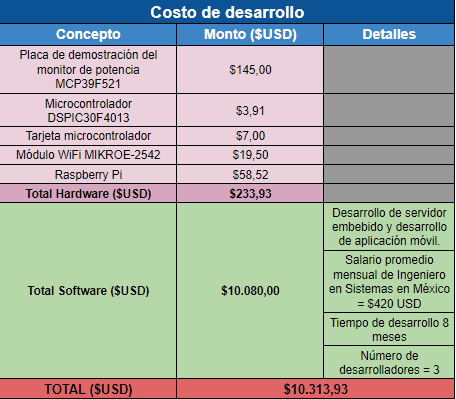
\includegraphics[scale=.8]{Capitulo3/img/CostoDesarrollo.PNG}
	\caption{Tabla de costo de desarrollo.}	\label{fig:CostoDesarrollo}
\end{figure} 




